\documentclass[oneside,12pt,a4paper]{template/SPSTemplate} % Default font size is 12pt, it can be changed here

\usepackage{silence}

\usepackage{amsmath} % mathematical fractions
\usepackage{lipsum}
\usepackage{array,multirow,graphicx,float}
\usepackage{csquotes}
\usepackage{biblatex}  %  sudo apt-get install texlive-bibtex-extra
\addbibresource{Main.bib}
\graphicspath{{./template/}{./Pictures/}}


\newcommand\TS{\rule{0pt}{2.6ex}}       % Top strut
\newcommand\BS{\rule[-1.2ex]{0pt}{0pt}} % Bottom strut


\creator{VERNER Adam}
\temacz{Dvoukanálový USB osciloskop}
\tema{Two-channel USB oscilloscope}
\supervisor{BUŠEK Jaroslav}
\vyuziti{Výukové účely v oboru mechatronika, programování, digitální zpracování signálu}
\abstrakt{Práce je zaměřena na vývoj zařízení sloužícího k digitálnímu zpracování analogového signálu}
\klicovas{Osciloskop, SystemVerilog, FPGA, USB, ADC, Pyhon, GTK, Altera}
\usage{Teaching purposes in the field of mechatronics, programming and digital signal processing}
\abstrakten{This work is focused on development of device used to digitally process an analogue signal}
\keywords{Oscilloscope, SystenVerilog, FPGA, USB, ADC, Python, GTK, Altera}
\podekovani{Děkuji vedoucímu práce za nulovou důvěru v mojí schopnost řádného dokončení projektu, která mě motivovala udělat něco víc, než všichni očekávají.\\
Také bych chtěl poděkovat svému otci, který mě již v útlém věku zainteresoval do digitálního světa, tím, že mě nechal rozbíjet vyřazené počítače.}

\newcommand\T{\rule{0pt}{2.6ex}}       % Top strut
\newcommand\B{\rule[-1.2ex]{0pt}{0pt}} % Bottom strut

\begin{document}
	\makebeginning

	\addcontentsline{toc}{chapter}{Obsah}
	\tableofcontents
	
	\chapter{Úvod}
	
	\chapter{Analogové zpracování signálů}
		Analogové zpracování signálů má mnoho výhod i nevýhod oprotoi tomu digitálnímu. Jednou z hlavních výhod je možnost zpracování daleko širšího pásma oproti digitálnímu zpracován. 

		Nejrychlejší transistor od firmy IBM je schopen spolehlivě pracovat až do frekvence 210 GHz, zatímco nejrychlejší ADC umí vstup pouze do 8Ghz se vzorkováním 6.4 Ghz a rozlišením 12 bitů \cite{(http://www.ti.com/product/adc12dl3200).}

		Avšak ve finále se používá kombinace obou metod, za pomocí analogových obvodů se signál před-připraví(před-zpracuje), tak aby se co dal nejlépe zaznamenávat pomocí ADC a poté složitější operace a analýza se provedou ve světě digitálním.

		\section{za použití pasivních součástek}
			Jak již název vypovídá, pomocí pasivních součástek se dá ze signálu pouze "ubírat." To znamená, že ze samotných pasivních součástek můžeme stavět pouze filtry, jsou ještě další aplikace, ale tam se bez křemíku neboejdeme.
			Pasivní součástky jsou Rezistory, kondenzátory a indukčnosti.

			V případě stejnosměrného signálu(stailního) má na výstup vliv pouze rezistor, kondenzátor se chová jako otevřený spoj a indukčnost se chová opačně, tudíž kontakty spouje.
			U AC signálu, už to tak jednoduhé není. Kondenzátory zadržují náboj, špičky vyhlazují, fázově všechno posouvají jedním směrem, zatímco cívky dělají skoro přesný opak. Naštěstí pro nás, všechno se chová podle jistých pravidel.

			\begin{itemize}
			
				\item děliče napětí
				\item filtry {\color{red} doplnit druhy}

			\emd{itemize}
			
		
		\section{za použití aktivních součástek}
	
		\section{Digitalizace spojitých signálů}
		
			\subsection{Vzorkování}
		Ve zpracování signálu se vzorkováním myslí převod časově spojitého signálu do oblasti času diskrétního. 
		Signál diskrétní v čase nemůže být, narozdní od spojitého, vyjádřen jako funkce, ale je vyjádřen jako posloupnost.
		Diskrétní signál může vzniknout dvěma způsoby:
		\begin{itemize}
			\item získáním hodnot spojitého signálu při konstantním, nebo proměnlivém času. \cite{discretization_oppenheim}
			\item pozorováním procesu založeném na diskrétním čase, např.: sledováním extrémních hodnot.
		\end{itemize}
		
		
		Rychlost vzorkování může být vyjádřena buď jako frekvence $ f_{vz} $ nebo jako perioda $ T_{vz} $.
		Závislost frekvence na periodě vzorkování je vyjádřena v následující rovnici:
		
		\begin{equation}
		f_{vz} = \frac{1}{T_{vz}}
		\end{equation}

	
		\subsubsection{Aliasing}
		Vycházející z anglického slova \textit{alias}, znamenající: falešné jméno, pseudonym, "jinak zvaný." 
	

		\textit{„Přesná rekonstrukce spojitého, frekvenčně omezeného signálu z jeho vzorků je možná tehdy, pokud byla vzorkovací frekvence vyšší než dvojnásobek nejvyšší harmonické složky vzorkovaného signálu.“}\cite{sampling_nyquist}
	
		\begin{figure}[H]
			\centering
			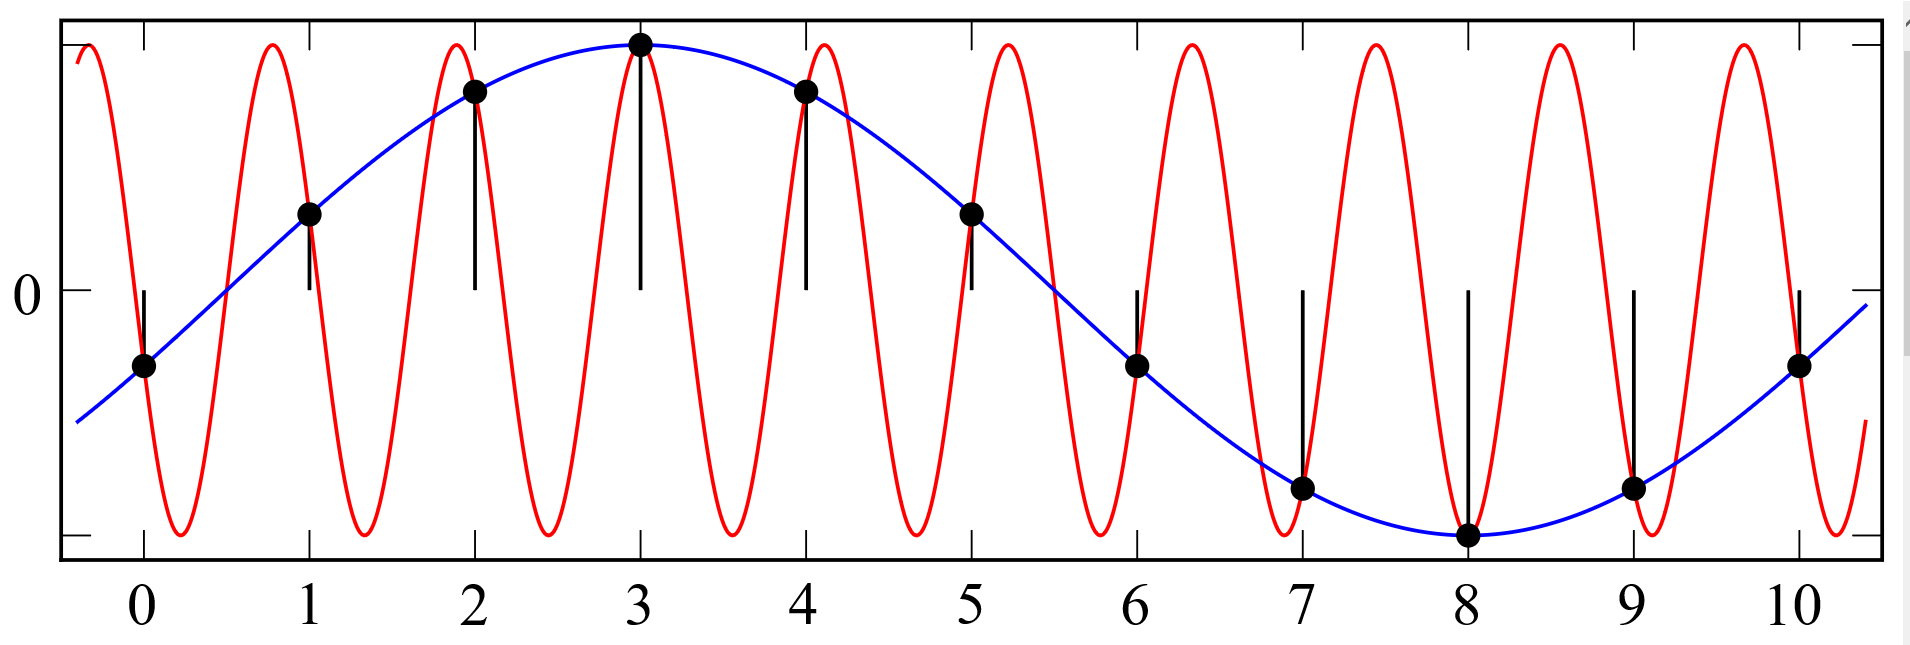
\includegraphics[width=\textwidth,keepaspectratio]{AliasingSines.eps}
			\caption{Červená - vzorkovaný signál. Modrá - rekonstruovaný signál}
			\label{img:aliasing}
		\end{figure}
	
	\chapter{Číslicové Zpracování signálu}

	V okolním světě se všechny signály vyskytují ve spojité formě, to znamená, že ať přibližujeme v jakékoliv dimenzi, vidíme pořád víc a víc detailů.
	
	

	\begin{table}[H]
		\catcode`\-=12
		\centering
		\newcolumntype{C}{ >{\centering\arraybackslash}m{0.3cm} }
		\newcolumntype{D}{ >{\centering\arraybackslash}m{2cm} }
		\begin{tabular}{|C|C|D|D|} \hline
			\multicolumn{2}{|c|}{\multirow{2}{*}{}} & \multicolumn{2}{c|}{ Čas }\\ \cline{3-4} 
			\multicolumn{2}{|c|}{} & Spojitý & nespojitý\\ \hline
			\multirow{2}{*}	{\rotatebox{90}{ hodnota \ \ }} & {\rotatebox{90}{\ Spojitá\ \ }} & spojitý & Kvantovaný \\ \cline{2-4} 
			& {\rotatebox{90}{\ Nespojitá\ \ }}  & Vzorkovaný  & Digitální \\ \hline
		\end{tabular}
	\end{table}
	
	
	

	
	\section{Programovatelné logické obvody}

	\section{Před-zpracování signálů}	
	
	\section{Zpracování signálů}
	
	\appendix
	
	\printbibliography
	
	\listoffigures
	\listoftables
	% seznam zkratek
	

\end{document}

